% !TeX program = pdflatex
\pdfoptionpdfminorversion=5
% \documentclass[9pt,hyperref={pdfpagelabels=false}]{beamer}
\documentclass[9pt, xcolor={dvipsnames}]{beamer}
% handout "deaktiviert" Animationen
%\documentclass[9pt,handout]{beamer}

\mode<presentation> {
    \usetheme{HHUD}
    \setbeamercovered{invisible}
}
\usepackage[ngerman]{babel}
\usepackage[utf8x]{inputenc}
\usepackage{times}
\usepackage{amsmath}
\usepackage{subfigure}
\usepackage{graphicx}
\usepackage{hyperref}
\usepackage{xmpmulti}
\usepackage{multirow}
\usepackage{appendixnumberbeamer}
\usepackage[normalem]{ulem}
\usepackage{mathabx}

\usepackage{textcomp}
\usepackage{listings}
\usepackage{color}
\usepackage{tabularx}

%%%%% https://github.com/cebe/pdfpc-latex-notes
% create a new file handle
\newwrite\pdfpcnotesfile

% open file on \begin{document}
\AtBeginDocument{%
	\immediate\openout\pdfpcnotesfile\jobname.pdfpc\relax
	\immediate\write\pdfpcnotesfile{[notes]}
}
% define a # http://tex.stackexchange.com/a/37757/10327
\begingroup
\catcode`\#=12
\gdef\hashchar{#}%
\endgroup
% define command \pnote{} that works exactly like not but
% additionally writes notes to file in pdfpc readable format
\newcommand{\pnote}[1]{%
	% keep normal notes working
	\note{#1}%
	% write notes to file
	\begingroup
	\let\#\hashchar
	\immediate\write\pdfpcnotesfile{\#\#\# \theframenumber}%
	\immediate\write\pdfpcnotesfile{\unexpanded{#1}}%
	\endgroup
}
% close file on \begin{document}
\AtEndDocument{%
	\immediate\closeout\pdfpcnotesfile
}
%%%%%


% background image
\usebackgroundtemplate{
\includegraphics[width=\paperwidth]
    {fig/background}}
% commands for low and high decoration in frame foot
\newcommand{\footdecorationlow}{\usebackgroundtemplate{
    
\includegraphics[width=\paperwidth]{fig/background_small}}}
\newcommand{\footdecorationhigh}{\usebackgroundtemplate{
    
\includegraphics[width=\paperwidth]{fig/background}}}

% Own commands:

 \AtBeginSection[] {
   \footdecorationhigh
   \begin{frame}<beamer>
     \thispagestyle{empty}
     \frametitle{Gliederung}
     \vspace{-5mm}
     \tableofcontents[currentsection]
   \end{frame}
   \footdecorationlow
 }

% % % % % % % %  CHANGE TOPIC AND AUTHOR INFORMATION HERE % % % % % % %
% HIER DEN TITEL DER ARBEIT EINTRAGEN                                                   
\title{Eine Toolbox zur Simulation und Visualisierung von Automaten und Grammatiken}
% HIER DEN NAMEN UND VORNAMEN EINTRAGEN
\author{Fabian Ruhland} 
% HIER DAS PR\"aSENTATIONSDATUM EINTRAGEN                                           
\date{27.10.2016}
% % % % % % % % % % % % % % % % % % % % % % % % % % % % % % % % % % % % 
\institute{Institut für Softwaretechnik und Programmiersprachen\\Heinrich-Heine-Universität Düsseldorf}
\subject{Informatik}

% % % % % % % % % % Own commands % % % % % % % %

%
% Hier beginnt das Dokument
%
\begin{document}

  \footdecorationhigh
  \begin{frame}
    \thispagestyle{empty}
    \titlepage
  \end{frame}

% Inhaltsverzeichnis - fuer kurze Vorträge eher weglassen
   \begin{frame}
     \thispagestyle{empty}
     \frametitle{Gliederung}
     \vspace{-5mm}
     \tableofcontents
   \end{frame}

% Fußzeile wieder niedrig setzen für normale Folien
   \footdecorationlow

% Ab hier werden die LaTeX-Dateien der einzelnen Abschnitte eingef\"ugt

\lstset{
	captionpos=b,
	breaklines=true,
}

\section{Zielsetzung}
\begin{frame}\frametitle{1 - Zielsetzung}
	\begin{itemize}
		\item Tools zum Lernen für Studenten von Theoretischer Informatik und Compilerbau bereitstellen
		\item Sowohl von der Konsole, als auch per grafischer Oberfläche bedienbar
		\item Leichte Erweiterbarkeit des Programms
		\item Programmiersprachen: Java, SableCC
	\end{itemize}
\end{frame}

\section{Umsetzung}
\begin{frame}\frametitle{2 - Umsetzung}
	\begin{itemize}
		\item Grammatiken:
		\begin{itemize}
			\item First-Mengen berechnen
			\item Follow-Mengen berechnen
			\item LL-Parser-Tabelle aufstellen
		\end{itemize}
		\pause
		\item Automaten:
		\begin{itemize}
			\item Entfernen von Epsilon-Übergängen
			\item Vervollständigen der Übergangsfunktion
			\item Umwandeln eines NFA in einen DFA
			\item Minimieren eines DFA
			\item Exportieren in GraphViz-Format (.dot-Datei)
		\end{itemize}
	\end{itemize}
\end{frame}

\begin{frame}\frametitle{2 - Umsetzung}
	\begin{itemize}
		\item Mit SableCC erstellte Parser zum Einlesen von Automaten und Grammatiken aus Textdateien
		\item Programm startet in Konsole; Mit Konsolenbefehlen können Dateien eingelesen und Algorithmen ausgeführt werden
		\item GUI wird per Konsolenbefehl gestartet; Automaten und Grammatiken sind hier vollständig editierbar
	\end{itemize}
\end{frame}

\begin{frame}\frametitle{2 - Umsetzung}
	\begin{itemize}
		\item Selbst entwickeltes Plugin-System zur Erweiterung der Toolbox:
		\begin{itemize}
			\item Interfaces um Konsole und GUI neue Funktionen hinzuzufügen (Plugins)
			\item Plugins werden zur Laufzeit geladen
			\item Wenig Kenntnis über meinen Code vorausgesetzt
		\end{itemize}
	\end{itemize}
\end{frame}

\section{Eingabegrammatiken}
\begin{frame}\frametitle{3 - Eingabegrammatiken}
	\begin{itemize}
		\item Selbst erdachtes Eingabeformat
		\item Parser wurden mit SableCC erstellt
		\item Automaten und Grammatiken werden in Textdateien gespeichert
	\end{itemize}
\end{frame}

\begin{frame}[fragile]\frametitle{3 - Eingabegrammatiken}
	{ \fontsize{20}{20} \selectfont \underline{Grammatiken}}
	\ \\
	\ \\
	\ \\
	\pause
	\begin{itemize}
		\item Erst werden Terminale, Nichtterminale und das Startsymbol definiert
        \begin{lstlisting}[frame=single]
{'a', 'b', 'c'; S, A, B; S}
        \end{lstlisting}
        \pause
        \item Anschließend werden die Produktionen aufgelistet
        \begin{lstlisting}[frame=single]
S --> 'A', 'b'
A --> 'A', 'a'
        \end{lstlisting}    
	\end{itemize}
\end{frame}

\begin{frame}[fragile]\frametitle{3 - Eingabegrammatiken}
		\begin{itemize}
		\item Vollständige Grammatik
		\begin{lstlisting}[frame=single]
{'a', 'b', 'c'; S, A, B; S}

S --> 'A', 'B'
A --> 'A', 'a'
A --> 'a'
B --> 'B', 'b'
B --> 'b'
	    \end{lstlisting}
		\end{itemize}
\end{frame}

\begin{frame}[fragile]\frametitle{3 - Eingabegrammatiken}
	{ \fontsize{20}{20} \selectfont \underline{Automaten}}
	\ \\
	\ \\
	\ \\
	\pause
	\begin{itemize}
		\item Erst werden Zustände, Startzustand und Endzustände definiert
		\begin{lstlisting}[frame=single]
{z0, z1, z2; z0; z2}
		\end{lstlisting}
		\pause
		\item Anschließend werden die Produktionen aufgelistet
		\begin{lstlisting}[frame=single]
z0 --'a','b'--> z1
		\end{lstlisting}    
	\end{itemize}
\end{frame}

\begin{frame}[fragile]\frametitle{3 - Eingabegrammatiken}
	\begin{itemize}
		\item Vollständiger Automat
		\begin{lstlisting}[frame=single]
{z0, z1, z2; z0; z2}

z0 --'a'--> z1
z1 --'a'--> z1
z1 --'b'--> z2
z2 --'b'--> z2
		\end{lstlisting}
	\end{itemize}
\end{frame}

\section{Live-Demo}
\begin{frame}\frametitle{4 - Live-Demo}
\end{frame}

\lstset{
	language=Java,
	breaklines=true,
	commentstyle=\color{OliveGreen},
	keywordstyle=\color{blue},
	stringstyle=\color{magenta}
}

\section{Plugins}
\begin{frame}\frametitle{5 - Plugins}
	\begin{itemize}
		\item Verschiedene Plugins für Konsole und GUI
		\item Müssen entsprechendes Interface implementieren und im richtigen Ordner liegen
		\item Werden vom Hauptprogramm zur Laufzeit geladen
	\end{itemize}
\end{frame}

\begin{frame}\frametitle{5 - Plugins}
	{ \fontsize{20}{20} \selectfont \underline{Plugins für die Konsole}}
	\ \\
	\ \\
	\ \\
	\pause
	\begin{itemize}
		\item Plugins liegen im Package \textit{CLIPlugins/}
		\item Implementieren das Interface \textit{CLIPlugin}
	\end{itemize}
\end{frame}

\begin{frame}[fragile]\frametitle{5 - Plugins}
	\begin{itemize}
		\item[] Das Interface \textit{CLIPlugin}
		\pause
		\begin{lstlisting}[frame=single, basicstyle=\tiny]
public interface CLIPlugin {

	//Gibt Aufrufnamen zurueck
	String[] getNames();
	
	//Prueft uebergebene Parameter
	boolean checkParameters(String[] parameters);
	
	//Gibt den Hilfetext zurueck
	String getHelpText();
	
	//Die eigentliche Funktion des Plugins
	Object execute(Object object, String[] parameters);
	
	//Klassentyp von 'object'
	Class inputType();
	
	//Klassentyp des Rueckgabewertes von 'execute'
	Class outputType();
	
	//true, wenn bei der Ausfuehrung von 'execute ein Fehler auftrat
	boolean errorFlag();
}
		\end{lstlisting}
	\end{itemize}
\end{frame}

\begin{frame}[fragile]\frametitle{5 - Plugins}
	{ \fontsize{12}{12} \selectfont Beispiel \textit{AutomatonLoadPlugin}}
	\pause
	\begin{itemize}
		\item[]
		\begin{lstlisting}[frame=single, basicstyle=\tiny]
public class AutomatonLoadPlugin implements CLIPlugin{

	private boolean errorFlag = false;
		\end{lstlisting}
		\pause
		\item[]
		\begin{lstlisting}[frame=single, basicstyle=\tiny]
	@Override
	public String[] getNames() { return new String[]{"la", "load-automaton"}; }
		\end{lstlisting}
		\pause
		\item[]
		\begin{lstlisting}[frame=single, basicstyle=\tiny]
	@Override
	public boolean checkParameters(String[] parameters) {
		//Dieses Plugin erwartet einen Parameter:
		//Den Pfad zur Datei, die es laden soll.
		
		if(parameters.length < 1) {
			System.out.println("Please enter a filename as parameter for this command!");
			return false;
		}
		return true;
	}
		\end{lstlisting}
	\end{itemize}
\end{frame}

\begin{frame}[fragile]\frametitle{5 - Plugins}
	\begin{itemize}
		\item[]
		\begin{lstlisting}[frame=single, basicstyle=\tiny]
    @Override
	public Object execute(Object object, String[] parameters) {
		errorFlag = false;
		Automaton automaton = null;
		try {
			//Datei zeilenweise einlesen und in der Variable 'file' speichern.
			//Anschliessend von 'AutomatonUtil.parse()' zu einem Automaten parsen lassen.
			String filename = parameters[0];
			BufferedReader automatonReader = new BufferedReader(new FileReader(filename));
			String file = "";
			String line;
			while ((line = automatonReader.readLine()) != null) {
				file = file + line + "\n";
			}
			automaton = AutomatonUtil.parse(file);
		} catch (FileNotFoundException e) {
			System.out.println("File not found!");
			errorFlag = true;
		} catch (IOException e) {
			System.out.println("Unable to read file!");
			errorFlag = true;
		} catch (ParserException e) {
			System.out.println("Error while parsing the file!");
			e.printStackTrace();
			errorFlag = true;
		} catch (LexerException e) {
			System.out.println("Error while parsing the file!");
			e.printStackTrace();
			errorFlag = true;
		}
		return automaton;
	}
}
		\end{lstlisting}
	\end{itemize}
\end{frame}

\begin{frame}[fragile]\frametitle{5 - Plugins}
	\begin{itemize}
		\item[]
		\begin{lstlisting}[frame=single, basicstyle=\tiny]
@Override
public Class inputType() {
	//'execute' erwartet keine Input-Objekt.
	return null;
}
	\end{lstlisting}
	\pause
	\item[]
	\begin{lstlisting}[frame=single, basicstyle=\tiny]
@Override
public Class outputType() {
	//'execute' gibt einen Automaten zurueck.
	return Automaton.class;
}
	\end{lstlisting}
	\pause
	\item[]
	\begin{lstlisting}[frame=single, basicstyle=\tiny]
@Override
public boolean errorFlag() {
	return errorFlag;
}
		\end{lstlisting}
	\end{itemize}
\end{frame}

\begin{frame}\frametitle{5 - Plugins}
	{ \fontsize{20}{20} \selectfont \underline{Plugins für die grafische Oberfläche}}
	\ \\
	\ \\
	\ \\
	\pause
	\begin{itemize}
		\item Plugins liegen im Package \textit{GUIPlugins/}
		\item Drei verschiedene Interfaces mit jeweils eigenen Packages:
		\begin{itemize}
			\item DisplayPlugin - Zur Darstellung von Objekten
			\item SimpleFunctionPlugin - Um der GUI einfache Funktionen hinzuzufügen
			\item ComplexFunctionPlugin - Um der GUI Funktionen mit wiederum eigener GUI hinzuzufügen
		\end{itemize}
	\end{itemize}
\end{frame}

\begin{frame}\frametitle{5 - Plugins}
	\begin{center}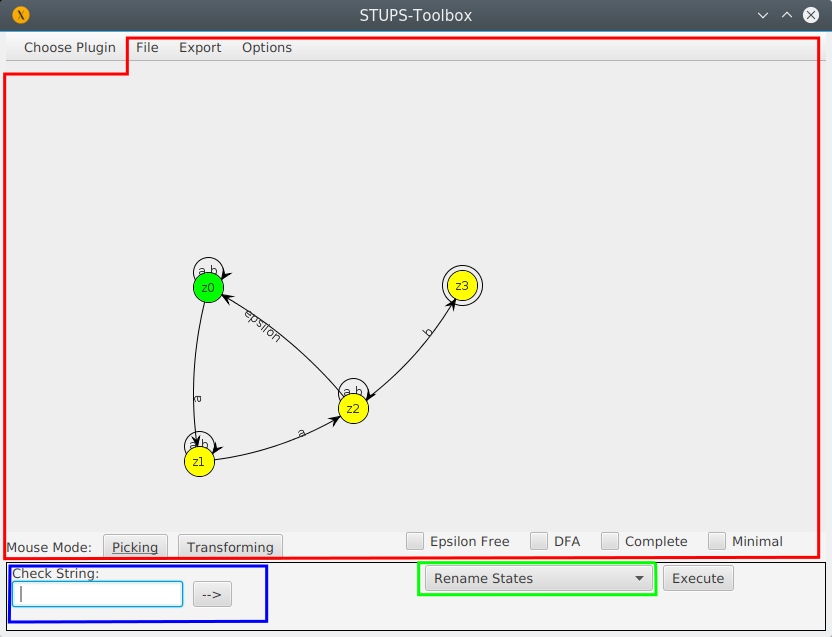
\includegraphics[width=0.6\textwidth]{fig/gui.png}\end{center}
	\begin{itemize}
		\item \textcolor{red}{\textbf{DisplayPlugin}}
		\item \textcolor{green}{\textbf{SimpleFunctionPlugin}}
		\item \textcolor{blue}{\textbf{ComplexFunctionPlugin}}
	\end{itemize}
\end{frame}

\begin{frame}[fragile]\frametitle{5 - Plugins}
	\begin{itemize}
		\item[] Das Interface \textit{DisplayPlugin}
		\begin{lstlisting}[frame=single, basicstyle=\tiny]
public interface DisplayPlugin {

//Gibt einen Java-FX Node zurueck, der in der GUI angezeigt wird
Node display(Object object);

//Anzeige aktualisieren
void refresh(Object object);

//Neues Objekt erstellen (File --> New)
Object newObject();

//Datei oeffnen und zu Objekt parsen (File --> Open)
Object openFile();

//Objekt in Datei speichern (File --> Save)
void saveFile(Object object);

//Zusaetzliche Menueobjekte fuer die Menueleiste der GUI
HashSet<Menu> menus(Object object, Node node);

//Name des Plugins (ChoosePlugin-Menue)
String getName();

//Klassentyp von 'object'
Class displayType();
}
		\end{lstlisting}
	\end{itemize}
\end{frame}

\begin{frame}[fragile]\frametitle{5 - Plugins}
	{ \fontsize{12}{12} \selectfont Beispiel \textit{GrammarGUI}}
	\begin{itemize}
		\pause
		\item[]
		\begin{lstlisting}[frame=single, basicstyle=\tiny]
public class GrammarExample implements DisplayPlugin {

	GridPane rootPane;
		\end{lstlisting}
		\pause
		\item[]
		\begin{lstlisting}[frame=single, basicstyle=\tiny]
	//Hilfsmethode, die eine Grammatik auf 'rootPane' darstellt.
	private void displayRules(Grammar grammar) {
		rootPane.getChildren().clear();
		
		//Ueber alle Nichtterminale der Grammatik iterieren und jede Produktion 'rootPane' hinzufuegen
		int i = 0;
		for(Nonterminal nonterminal : GrammarUtil.getNonterminalsInOrder(grammar)) {
			for(ArrayList<Symbol> symbolList : nonterminal.getSymbolLists()) {
				StringBuilder sb = new StringBuilder();
				Iterator<Symbol> it = symbolList.iterator();
				while(it.hasNext()) {
					sb.append(it.next().getName());
					if(it.hasNext()) {
						sb.append(", ");
					}
				}
			
				rootPane.add(new Label(nonterminal.getName()), 0, i);
				rootPane.add(new Label("-->"), 1, i);
				rootPane.add(new Label(sb.toString()), 2, i);
				i++;
			}
		}
	}
		\end{lstlisting}
	\end{itemize}
\end{frame}

\begin{frame}[fragile]\frametitle{5 - Plugins}
	\begin{itemize}
		\item[]
		\begin{lstlisting}[frame=single, basicstyle=\tiny]
	@Override
	public Node display(Object object) {
		Grammar grammar = (Grammar) object;
		
		//'rootPane' initialisieren und einrichten
		rootPane = new GridPane();
		rootPane.setAlignment(Pos.CENTER);
		rootPane.setHgap(10);
		rootPane.setVgap(5);
		
		//'displayRules' aufrufen um Grammatik auf 'rootPane' anzuzeigen
		displayRules(grammar);
		return rootPane;
	}
		\end{lstlisting}
		\pause
		\item[]
		\begin{lstlisting}[frame=single, basicstyle=\tiny]
	@Override
	public void refresh(Object object) {
		displayRules((Grammar) object);
	}
		\end{lstlisting}
	\end{itemize}
\end{frame}

\begin{frame}[fragile]\frametitle{5 - Plugins}
	\begin{itemize}
		\item[]
		\begin{lstlisting}[frame=single, basicstyle=\tiny]
	@Override
	public Object newObject() {
	return new Grammar();
	}
		\end{lstlisting}
		\pause
		\item[]
		\begin{lstlisting}[frame=single, basicstyle=\tiny]
	@Override
	public Object openFile() {
		//Dialog zum Auswaehlen einer Datei anzeigen
		FileChooser chooser = new FileChooser();
		chooser.setTitle("Open file");
		File selectedFile = chooser.showOpenDialog(new Stage());
		String fileInput = "";
		try {
			//Datei einlesen und von 'GrammarUtil.parse()' zu einer Grammatik parsen lassen
			BufferedReader reader = new BufferedReader(new FileReader(selectedFile.getName()));
			String line;
			while ((line = reader.readLine()) != null) {
				fileInput = fileInput + line + "\n";
			}
			return GrammarUtil.parse(fileInput);
		} catch (Exception e) {
			Alert alert = new Alert(Alert.AlertType.ERROR);
			alert.setTitle("STUPS-Toolbox");
			alert.setHeaderText("Error while opening the file!");
			alert.showAndWait();
			return null;
		}
	}
		\end{lstlisting}
	\end{itemize}
\end{frame}

\begin{frame}[fragile]\frametitle{5 - Plugins}
	\begin{itemize}
		\item[]
		\begin{lstlisting}[frame=single, basicstyle=\tiny]
	@Override
	public void saveFile(Object object) {
		FileChooser chooser = new FileChooser();
		chooser.setTitle("Save file");
		File selectedFile = chooser.showSaveDialog(new Stage());
		if(selectedFile != null) {
			GrammarUtil.save((Grammar) object, selectedFile.getAbsolutePath());
		}
	}
		\end{lstlisting}
		\pause
		\item[]
		\begin{lstlisting}[frame=single, basicstyle=\tiny]
	@Override
	public HashSet<Menu> menus(Object object, Node node) {
		MenuItem helpItem = new MenuItem("Help");
		MenuItem aboutItem = new MenuItem("About Plugin");
		
		helpItem.setOnAction(event -> {
			Alert alert = new Alert(Alert.AlertType.INFORMATION);
			alert.setTitle("STUPS-Toolbox");
			alert.setHeaderText("This is just a simple example plugin,\nthat displays all productions of the loaded grammar.");
			alert.showAndWait();
		});
		
		aboutItem.setOnAction(event -> {
			Alert alert = new Alert(Alert.AlertType.INFORMATION);
			alert.setTitle("STUPS-Toolbox");
			alert.setHeaderText("Grammar Example Plugin v1.0");
			alert.showAndWait();
		});
		
		Menu aboutMenu = new Menu("Help");
		aboutMenu.getItems().addAll(helpItem, aboutItem);
		return new HashSet<>(Arrays.asList(aboutMenu));
	}
		\end{lstlisting}
	\end{itemize}
\end{frame}

\begin{frame}[fragile]\frametitle{5 - Plugins}
	\begin{itemize}
		\item[]
		\begin{lstlisting}[frame=single, basicstyle=\tiny]
	@Override
	public String getName() {
		return "Grammar Example";
	}
		\end{lstlisting}
		\pause
		\item[]
		\begin{lstlisting}[frame=single, basicstyle=\tiny]
	@Override
	public Class displayType() {
		//Plugin zeigt Grammatiken an
		return Grammar.class;
	}
}
		\end{lstlisting}
	\end{itemize}
\end{frame}

\section{Makefile}
\begin{frame}[fragile]\frametitle{6 - Makefile}
	\begin{itemize}
		\item Mit Hinsicht auf Erweiterbarkeit der Toolbox geschrieben
		\item Kompiliert automatisch alle .java- und .scc-Dateien in allen Unterordnern in \textit{src/}
		\item Fügt automatisch alle .jar-Dateien in allen Unterordnern in \textit{lib/} dem Java-Classpath hinzu
		\item Lädt SableCC automatisch herunter.
	\end{itemize}
\end{frame}

\begin{frame}[fragile]\frametitle{6 - Makefile}
	{ \fontsize{12}{12} \selectfont Funktionen des Makefiles}
	\begin{itemize}
		\item \textit{build}: Kompiliert den Quellcode
		\item \textit{make unix}: Kompiliert und erstellt ausführbare .sh-Datei
		\item \textit{make windows}: Kompiliert und erstellt ausführbare .bat-Datei
		\item \textit{make package}: Kompiliert, erstellt ausführbare .sh- und .bat-Dateien und packt alles in .tar-Datei
		\pause
		\item \textit{make doc}: Generiert javadoc-Dokumentation
		\item \textit{make text}: Generiert die Bachelorarbeit als pdf-Datei
		\item \textit{make presentation}: Generiert diese Präsentation als pdf-Datei
		\pause
		\item \textit{make all}: Führt package, doc, text und presentation nacheinander aus
		\pause
		\item \textit{make clean}: Löscht alle generierten Dateien
		\item \textit{make mrproper}: Löscht alle generierten Dateien und die runtergeladene Version von SableCC
		\pause
		\item \textit{make develope}: Generiert die Parser-Dateien im Ordner \textit{src/}
		\item \textit{make clean\_develope}: Löscht die generierten Parser-Dateien im Ordner \textit{src/}
	\end{itemize}
\end{frame}

\section{Fazit}
\begin{frame}\frametitle{7 - Fazit}
	\begin{itemize}
		\item Visualisierung von Automaten hilfreich für Anfänger
		\item Schrittweises Durchgehen eines Eingabewortes macht Funktionsweise eines Automaten leichter nachvollziehbar
		\item Als Unterstützung für Übungsaufgaben einsetzbar (lässt sich jedoch auch leicht missbrauchen)
		\item Durch modularen Aufbau leicht erweiterbar ohne zukünftige Entwickler einzuschränken
	\end{itemize}
\end{frame}

\begin{frame}\frametitle{8 - Danke}
	\begin{itemize}
		\item Danke für Ihre Aufmerksamkeit!
		\pause
		\item Fragen, Anmerkungen und Bugs an \href{mailto:Fabian.Ruhland@uni-duesseldorf.de}{\nolinkurl{Fabian.Ruhland@uni-duesseldorf.de}}
	\end{itemize}
\end{frame}

% % % % % % % % % Ende der eingef\"ugten LaTeX-Dateien % % % % % % % % %

\end{document}

%
% Hier endet das Dokument
%
